\documentclass[12pt]{article}
\usepackage[letterpaper, margin=1in, headheight=105pt]{geometry}
\usepackage{graphicx}
\usepackage{xcolor}
\usepackage{minted}
\usepackage{comment}
\usemintedstyle{manni}
\pagestyle{empty}

\begin{document}
\begin{comment}
\setcounter{section}{1}
\section{Homework Coding Part}
\setcounter{subsection}{1}
\subsection{Bayesian Spam Filtering}
The test error for Bayesian classifier is 11.00\%, while the majority class predictor has test error 38.56\%.
So we con conclude that the Bayesian classifier is working.
\inputminted[frame=single,framesep=10pt,linenos,xleftmargin=\parindent]{octave}{./hw2/problem2/Bayesian_spam_filtering.m}
\setcounter{subsection}{3}
\subsection{Handwritten digit classification with logistic regression}
The test error is 5.40\%.
My termination criterion is
\[ \frac{||\theta_{t+1}-\theta_{t}||}{||\theta_t||}<0.001 \]
The value of the objective function at the optimum is \(6381.5\).
Since the logistic regression rely on \(\eta(x)\) which is a probability, we take the difference between these probabilities and the threshold \(\frac{1}{2}\), and take the absolute value.
\[ \left|\eta(x)-\frac{1}{2}\right| \]
The larger this value is, the more confident the regression classifier is about its prediction.
\inputminted[frame=single,framesep=10pt,linenos,xleftmargin=\parindent]{octave}{./hw2/problem4/Handwritten_digit_classification.m}
\begin{figure}
    \centering
    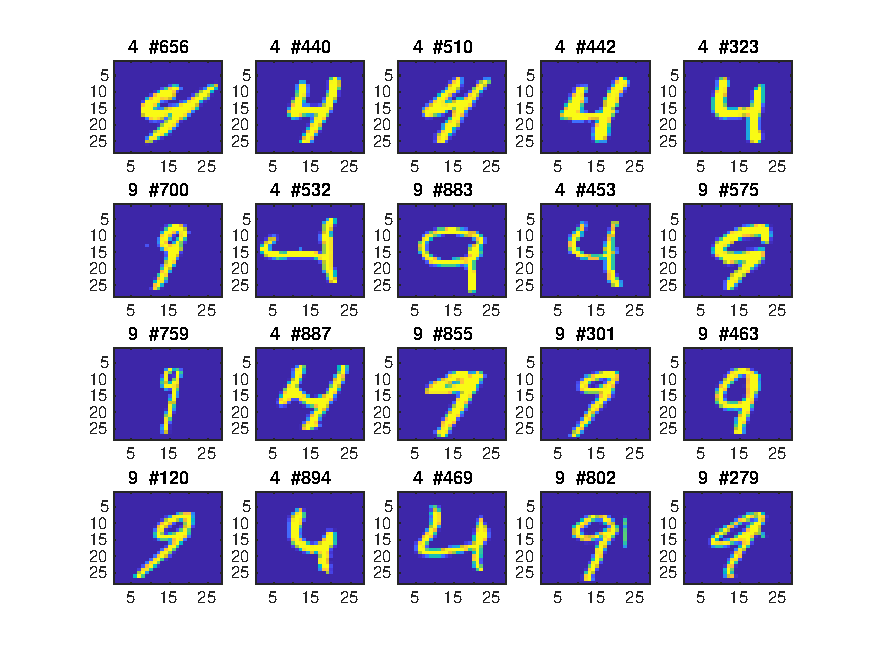
\includegraphics[width=0.85\textwidth]{./hw2/problem4/hw2p4b.pdf}
    \caption{Top 20 mis-classified images}
\end{figure}
\end{comment}

\setcounter{section}{2}
\section{Homework Coding Part}
\subsection{Linear Regression}
\inputminted[frame=single,framesep=10pt,linenos,xleftmargin=\parindent]{octave}{./hw3/problem1/Linear_regression.m}
The mean square error for ordinary linear regression is \(22.2826\).
The mean square error for regularized least squares regression is \(21.4859\).
The predicted response at the input \(x=[100, 100]\) is \(24.4581\).
The regularized least squares regression (Ridge) has parameter
\[ w=[ 0.6487, -0.0632]^T \hspace{2em} b=-34.0834 \]
\subsection{Robust Regression}
In order to be consistent with the higher dimension case, I denote \(\theta=[b, w]^T\), \(\tilde{x}_i=[1; x_i]\).
The majoring function is
\[ \bar{J} (\theta;\theta_t)=\sum_{i=1}^{n}\left[\rho(y_i-\tilde{x}_i^T\theta_t)-\frac{y_i-\tilde{x}_i^T\theta_t}{2}\rho'(y_i-\tilde{x}_i^T\theta_t) \right]+\frac{1}{2}\sum_{i=1}^{n}\frac{\rho'(y_i-\tilde{x}_i^T\theta_t)}{y_i-\tilde{x}_i^T\theta_t}\left(y_i-\tilde{x}_i^T\theta\right) \]
The first sum doesn't contain \(\theta\), so it has nothing to do with mininizing.
The second sum is exactly the reweighted least squares, as it can be written as
\[ \frac{1}{2}(y-\tilde{x}^T\theta)^T C (y-\tilde{x}^T\theta) \hspace{1em}\textrm{where } C=\texttt{diag}\left(\frac{\rho'(y_i-\tilde{x}_i^T\theta_t)}{y_i-\tilde{x}_i^T\theta_t}\right) \]
Thus, the iteration becomes
\[ \theta_{t+1}=\left(\tilde{x}^TC\tilde{x}\right)^{-1}\tilde{x}^TCy \]
Hence, the majoring-mininizing algorithm can be understood as ``iteratively reweighted least squares''.
It achieves robustness by assigning \emph{lower} weights for outliers and \emph{higher} weights for inliers.
As we can see, by picking specific \(\rho\) with \(\rho(r)=\sqrt{1+r^2}+1\), we have its derivative
\[ \rho'(r)=\frac{r}{\sqrt{1+r^2}} \]
Then, the weights are
\[ \frac{\rho'(r_{t,i})}{r_{t_i}}=\frac{1}{\sqrt{1+r_{t,i}^2}}=\frac{1}{\sqrt{1+\left(y_i-\tilde{x}_i^T\theta_t\right)^2}} \]
Thus, the outliers have less weights and inliers have more weights.
\begin{figure}[htbp]
    \centering
    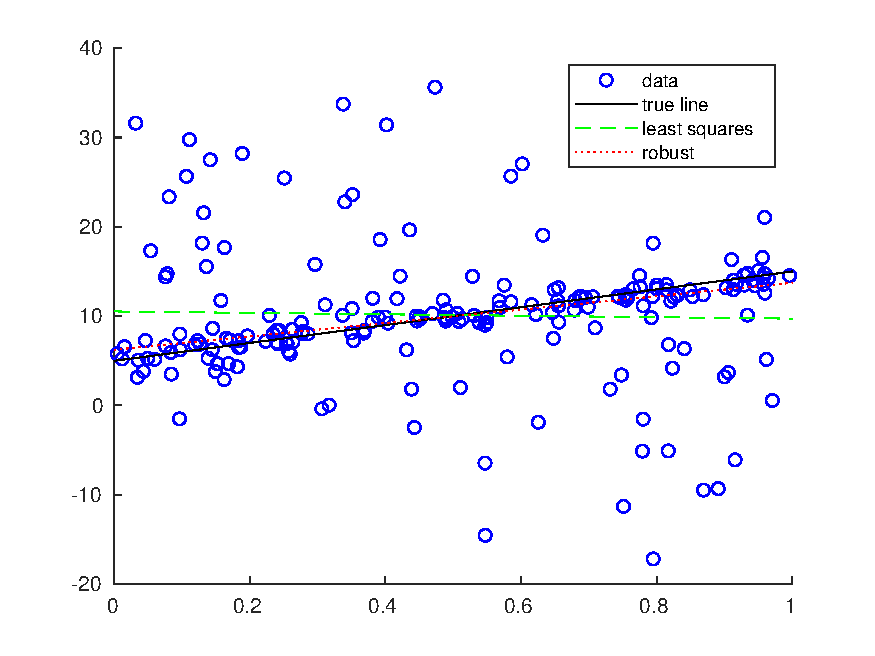
\includegraphics[width=0.85\textwidth]{./hw3/problem2/hw3p2.pdf}
    \caption{Data, true line, OLS estimate, robust estimate}
\end{figure}
The parameters from MM algorithm and ordinary linear regression are
\begin{center}
\begin{tabular}{c|cc}
    & \(w\) & \(b\) \\ \hline
    robust & \(7.4933\) & \(6.2352\) \\ \hline
    ordinary & \(-0.8061\) & \(10.5285\)
\end{tabular}
\end{center}
\inputminted[frame=single,framesep=10pt,linenos,xleftmargin=\parindent]{octave}{./hw3/problem2/Robust_regression.m}
\end{document}